\documentclass{article}
\usepackage{xcolor}
\usepackage{array}
\usepackage{graphicx}
\usepackage{multirow}
\title{GST 108: Introduction to Quantitative Reasoning}
\date{2021 - 11 - 18}
\author{Nnadiukwu Miracle}
\begin{document}
	\pagecolor{white}
	\pagenumbering{gobble}
	\maketitle
	\newpage
	\pagenumbering{arabic}
	\centering
	\section*{LOGIC GATES}
		\begin{table}[h!]
			\begin{tabular}{m{4cm} m{10cm}}
				\color{blue}
				{\LARGE\textbf{A logic gate is a building block of a digital circuit which is at the heart of any computer operation.}}	 & 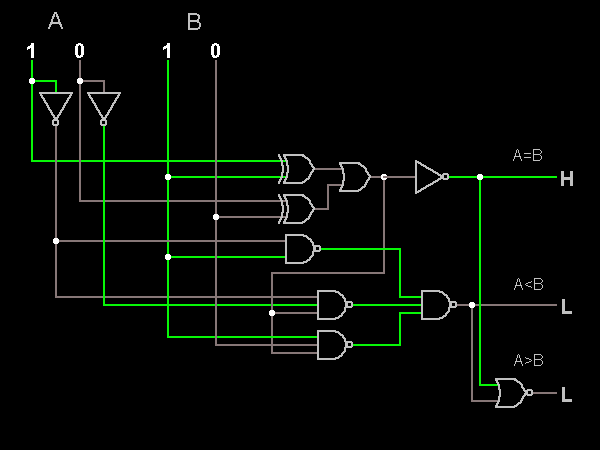
\includegraphics[width=1\linewidth]{circuit.png} \\
			\end{tabular}
		\end{table}
	\newpage
	\section*{LOGIC GATES}
	\begin{table}[h!]
		\begin{tabular}{m{4cm} m{10cm}}
			\color{blue}
			{\LARGE\textbf{Behind every digital system is a logic gate.
			}}	 & 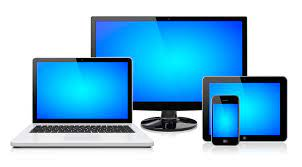
\includegraphics[width=1\linewidth]{devices.jpg} \\
		\end{tabular}
	\end{table}
\newpage
\section*{LOGIC GATES}
\begin{table}[h!]
	\begin{center}
		\begin{tabular}{c c c}
			\multicolumn{3}{m{12cm}}{\LARGE{\textbf {Logic gates perform logical operations that take binary input (0s and 1s) and produce  a single binary output. They are used in most electronic device including :}}} \\
			 & &  \\
			\color{red}{\Large \textbf{Smartphones}} & \color{green}{\Large \textbf{Tablets}} & \color{blue}{\Large \textbf{Memory devices}}\\
			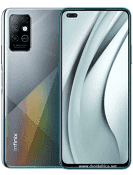
\includegraphics[width=0.3\linewidth]{phone.png} & 
\includegraphics[width=0.3\linewidth]{tablet.png} & 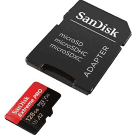
\includegraphics[width=0.3\linewidth]{memcard.png} \\
		\end{tabular}
	\end{center}
\end{table}
	\newpage
\section*{LOGIC GATES}
{\LARGE{\textbf {Now think of a logic gate like a light switch, it is either in an ON or OFF position. Similarly, the input output terminals are always in one of two binary positions false(0) and true(1). Each gate has its own logic or set of rules that determines how it acts based on multiple inputs outlined in a truth table.}}} 
\newpage
\section*{LOGIC GATES}
{\LARGE{\textbf {Combining 10s, 1000s or millions of logic gates makes it possible for a computer to perform highly complex operations and tasks at ever increasing speeds.
}}} 
\newpage
\section*{LOGIC GATES}
{\LARGE{\textbf {A gate is a basic electronic circuit which operates on one or more signals to produce an output signal. 
	\section*{Logic gates are digital circuits constructed from diodes, transistors, and resistors connected in such a way that the circuit output is the result of a basic logic operation \color{green}(OR, AND, NOT) \color{black}performed on the inputs.}
}}} 
\newpage
\section*{TYPES OF LOGIC GATES}
	{\LARGE{\textbf {Fundamental gates are \color{red}AND\color{black}, \color{red} OR \color{black}and \color{red}NOT
}}} 
\begin{table}[h!]
	\begin{center}
		\begin{tabular}{c c c}
			\multicolumn{3}{m{36cm}}{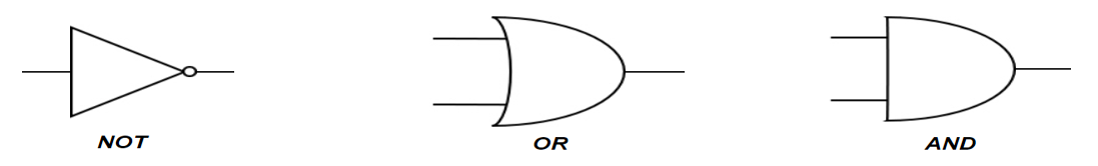
\includegraphics[width=0.3\linewidth]{gates.png}}\\
		\end{tabular}
	\end{center}
\end{table}
		{\LARGE{\textbf {Derived Gates are \color{red}NAND\color{black}, \color{red}NOR\color{black}, \color{red}XOR \color{black}and \color{red}XNOR \color{black}(derived from the fundamental gates)		
			}}} 
		
\end{document}

